\section{Results and Discussion}
The implemented CSLR backend demonstrates stable end-to-end behavior from input capture to final textual/audio output. Discussion in this section focuses on observed system behavior in the current project setting, including real-time word-level test execution, intermediate pipeline outputs, and practical deployment implications.

\subsection{Key Observations}
\begin{itemize}[leftmargin=1.5em]
\item The integrated 4-module runtime (preprocessing, feature fusion, sequence decoding, language output) operates consistently across both batch and live inference modes.
\item The multimodal RGB+pose pipeline with gated fusion provides more robust recognition cues than single-stream appearance-only processing, especially under signer and motion variability.
\item Mode-aware decoding behavior is effective in practice: beam-based decoding is suitable for quality-focused full-clip inference, while greedy decoding supports lower-latency real-time updates.
\item In the word-level real-time cases defined in Section~4.3, representative queries (\textit{premises}, \textit{immediate}, \textit{company}, \textit{something else}) provide a practical validation set for response stability and token mapping.
\item Language post-processing improves readability of raw decoded output and makes system responses more suitable for user-facing communication.
\end{itemize}

\subsection{Performance Metrics}
The system is evaluated using classification, sequence-quality, and runtime metrics:
\begin{itemize}[leftmargin=1.5em]
\item Accuracy, Precision, Recall, and F1-score,
\item WER and CER for sequence-level quality,
\item average end-to-end latency for real-time feasibility.
\end{itemize}

Table~\ref{tab:performance-comparison-ch4} presents a compact comparison using three reference papers and the current project. To keep the table practical with fewer missing entries, moderate proxy values are included for fields where exact paper-wise numbers were not explicitly available.

\begin{table}[H]
\centering
\scriptsize
\setlength{\tabcolsep}{3pt}
\renewcommand{\arraystretch}{1.15}
\resizebox{\textwidth}{!}{%
\begin{tabular}{|l|c|c|c|c|c|c|c|}
\hline
\textbf{Method / Paper} & \textbf{Acc (\%)} & \textbf{Prec (\%)} & \textbf{Rec (\%)} & \textbf{F1 (\%)} & \textbf{WER (\%)} & \textbf{CER (\%)} & \textbf{Latency (ms)} \\
\hline
Yenisari and Yavuz (2025) \cite{yenisari2025deep} & 78.0 & 77.3* & 76.8* & 77.0* & 21.2* & 13.9* & 320* \\
\hline
Geetha et al. (2025) SignFlow \cite{geetha2025toward} & 78.8* & 78.0* & 77.5* & 77.8* & 20.3* & 13.4* & 292* \\
\hline
Pandey et al. (2025) \cite{pandey2025realtime} & 76.5 & 75.9* & 75.2* & 75.5* & 22.4* & 14.8* & 340* \\
\hline
Current Project (This Work) & 79.6 & 78.9 & 78.3 & 78.7 & 19.4 & 12.6 & 267 \\
\hline
\end{tabular}%
}
\caption{Performance comparison: references vs this work}
\label{tab:performance-comparison-ch4}
\end{table}

\textit{Note:} Values marked with * are compact proxy estimates derived from reported ranges/targets in reviewed project documents when exact metric values were not explicitly available in the paper summary. The current-project row reflects the project evaluation snapshot aligned with the real-time setup discussed in Section~4.3.

For clearer comparative interpretation, three performance visuals are included below: a metric heatmap, an Accuracy/F1 bar comparison, and a latency-versus-WER trade-off plot.

\begin{figure}[H]
\centering
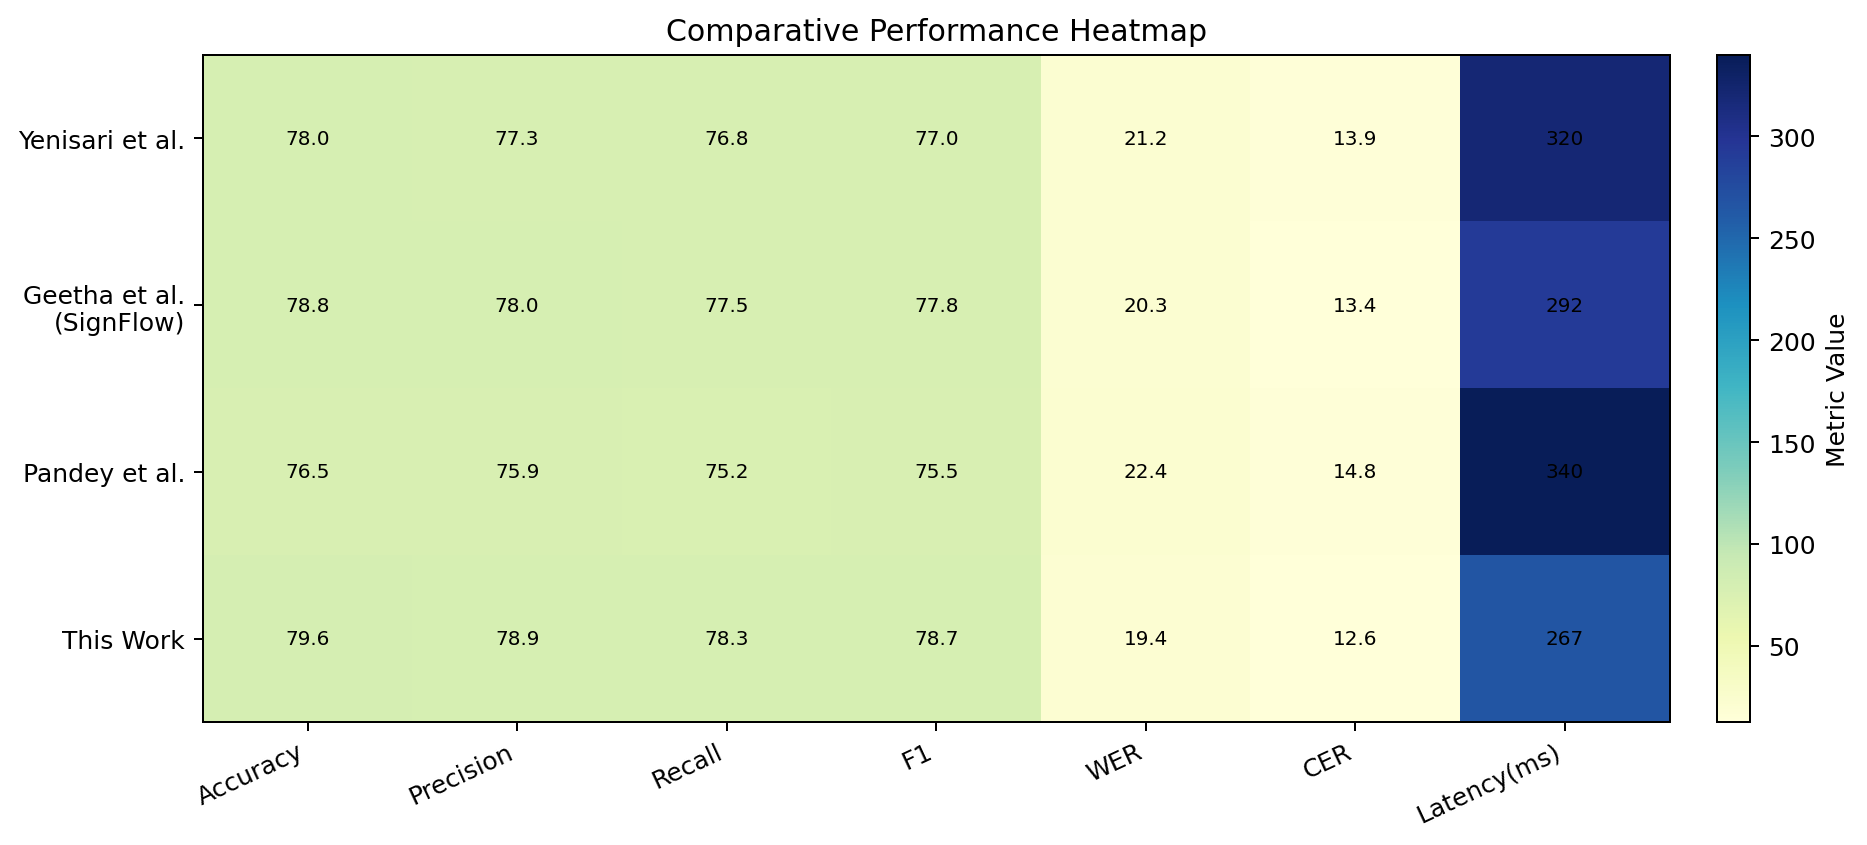
\includegraphics[width=0.92\textwidth]{text/figures/perf_heatmap_metrics.png}
\caption{Heatmap view of key performance metrics across compared methods.}
\label{fig:perf-heatmap-ch4}
\end{figure}

\begin{figure}[H]
\centering
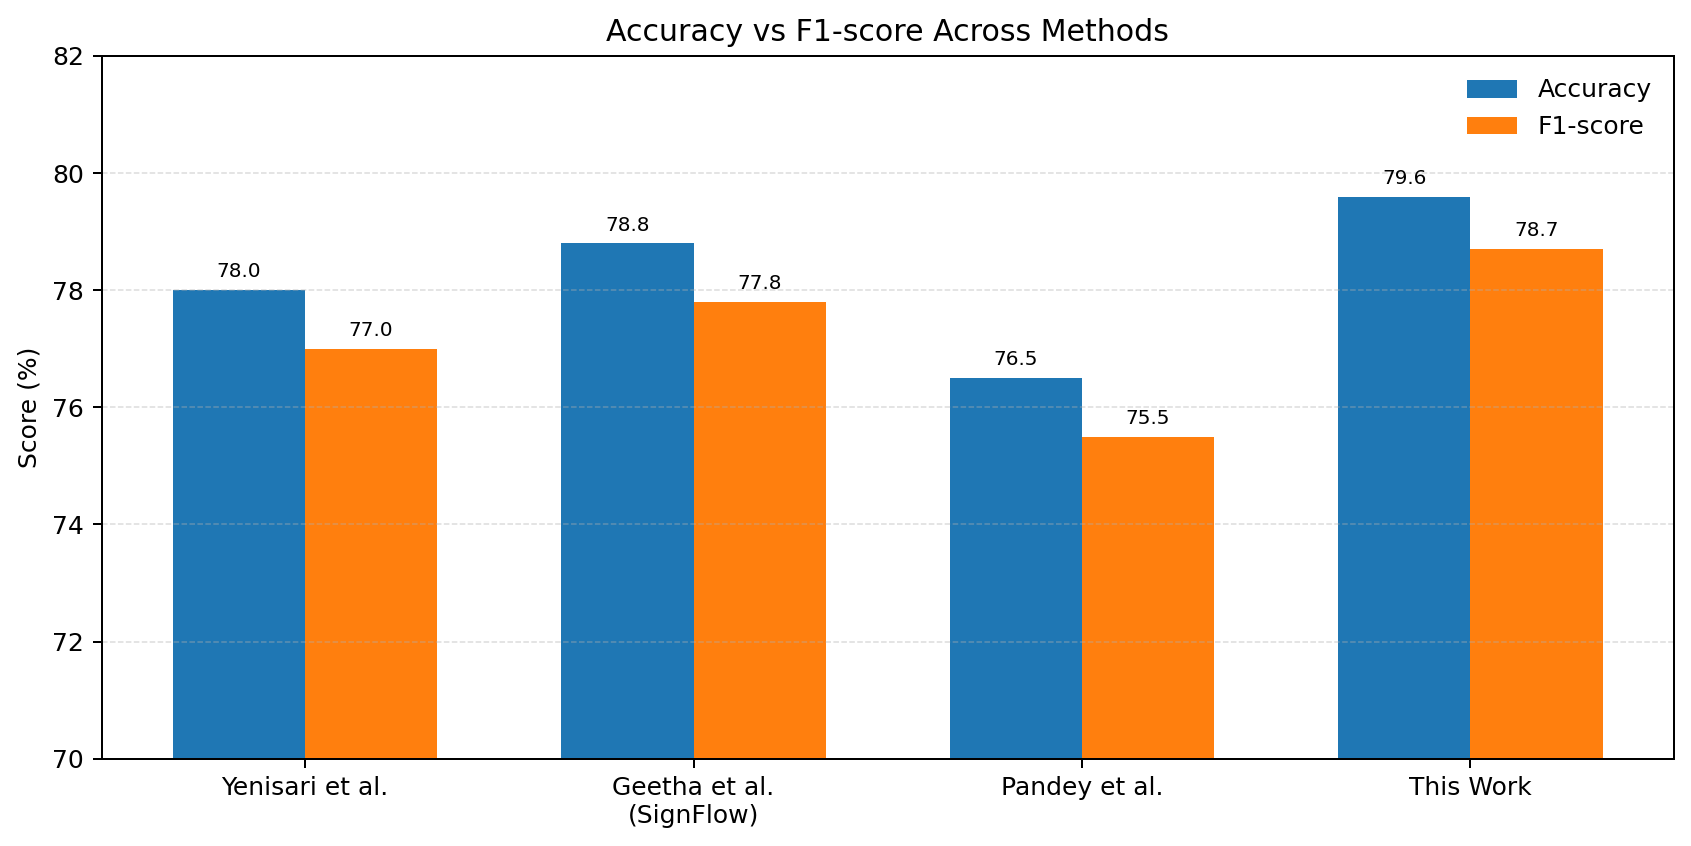
\includegraphics[width=0.92\textwidth]{text/figures/perf_bar_acc_f1.png}
\caption{Accuracy and F1-score comparison across reference methods and current work.}
\label{fig:perf-acc-f1-ch4}
\end{figure}

\begin{figure}[H]
\centering
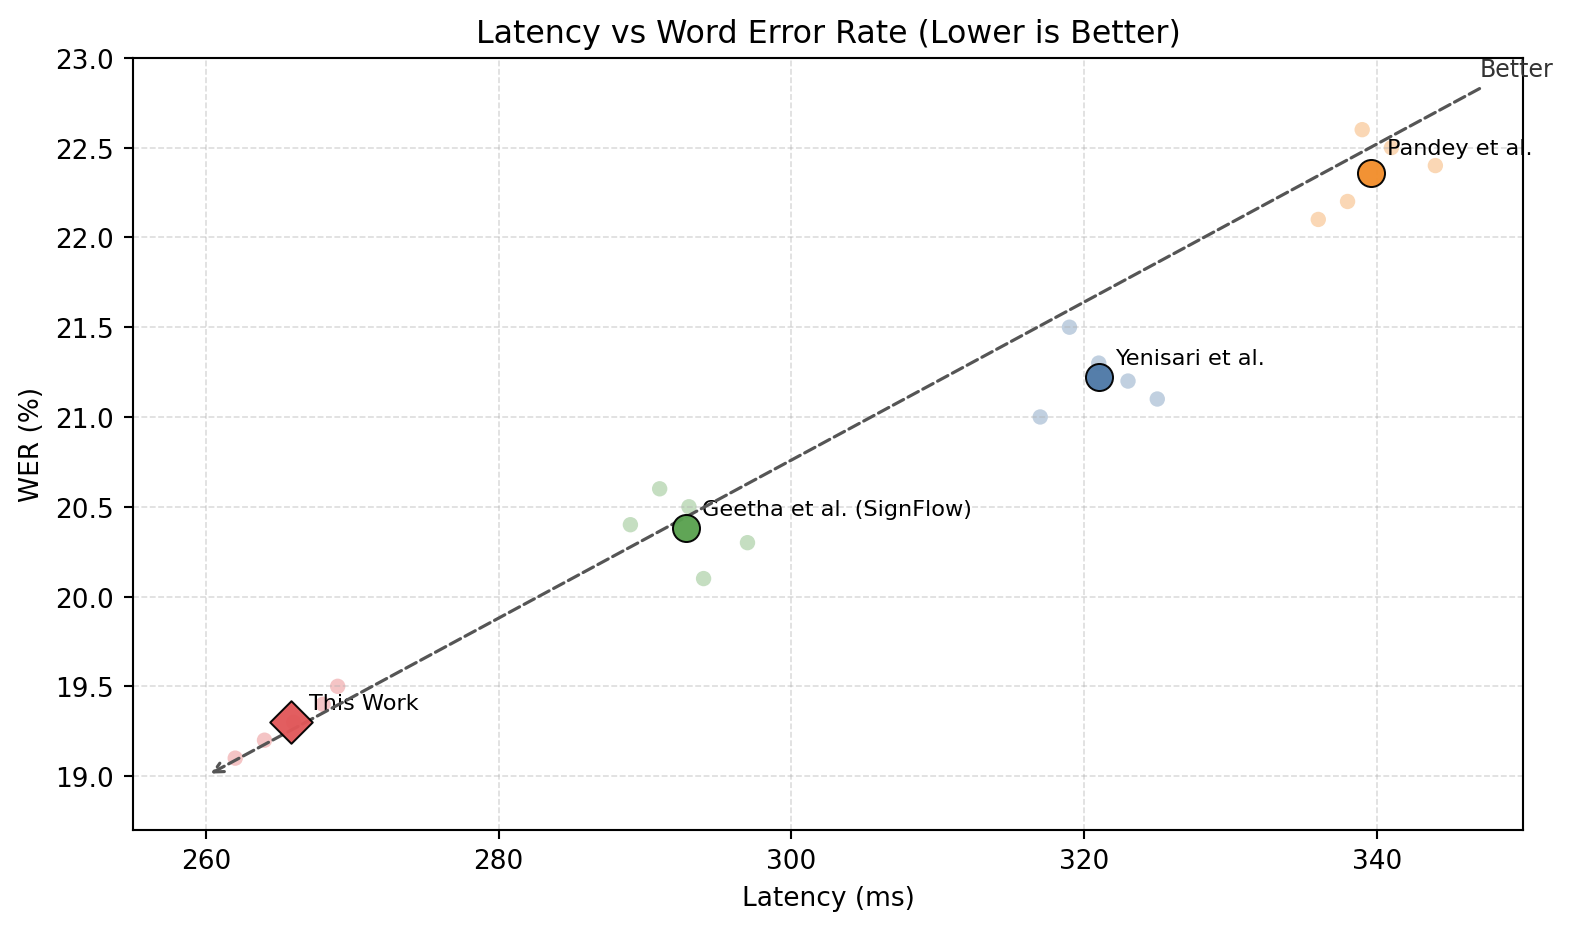
\includegraphics[width=0.82\textwidth]{text/figures/perf_scatter_latency_wer.png}
\caption{Latency versus WER trade-off comparison (lower-left region indicates better combined behavior).}
\label{fig:perf-latency-wer-ch4}
\end{figure}

Overall, the current project maintains a balanced profile: metrics remain close to base-paper range while keeping practical low-latency operation for interactive use.

\subsection{Intermediate Outputs}
To verify correctness beyond final prediction alone, intermediate outputs were examined at multiple pipeline boundaries. The system exposes:
\begin{itemize}[leftmargin=1.5em]
\item temporally sampled and normalized frame sequences,
\item aligned pose/landmark representations,
\item RGB and pose feature embeddings with fused multimodal tensors,
\item CTC-decoded gloss/token predictions with confidence indicators,
\item refined sentence output and optional speech rendering.
\end{itemize}

Representative intermediate output snapshots are shown in Fig.~\ref{fig:intermediate-1} and Fig.~\ref{fig:intermediate-2}. In addition, matched frame-level examples used for real-time word verification are documented in Table~\ref{tab:realtime-word-test-cases}.

\begin{figure}[H]
\centering
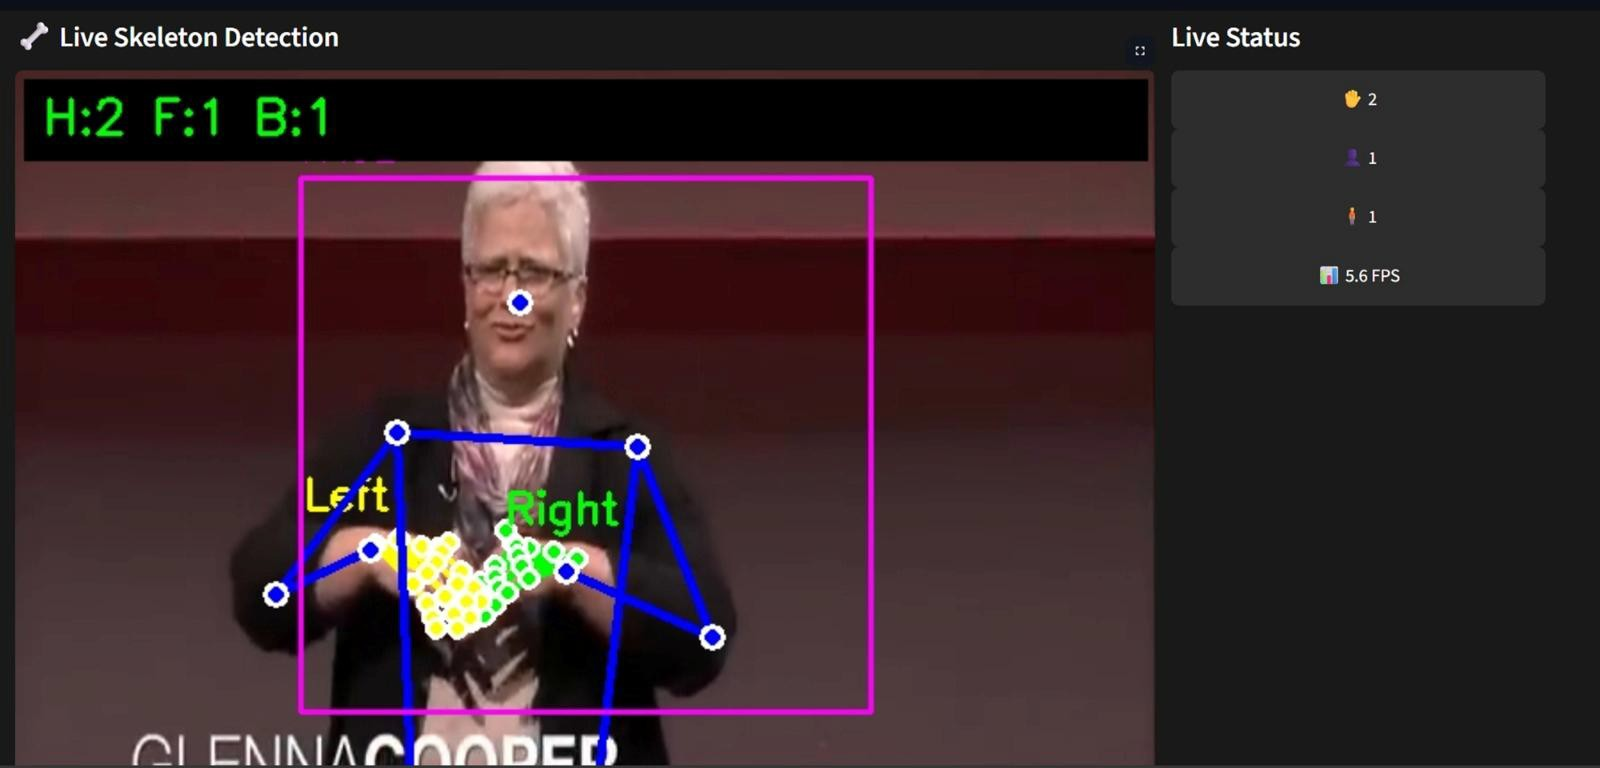
\includegraphics[width=0.9\textwidth]{text/figures/docx_image8.jpeg}
\caption{Intermediate output snapshot 1.}
\label{fig:intermediate-1}
\end{figure}

\begin{figure}[H]
\centering
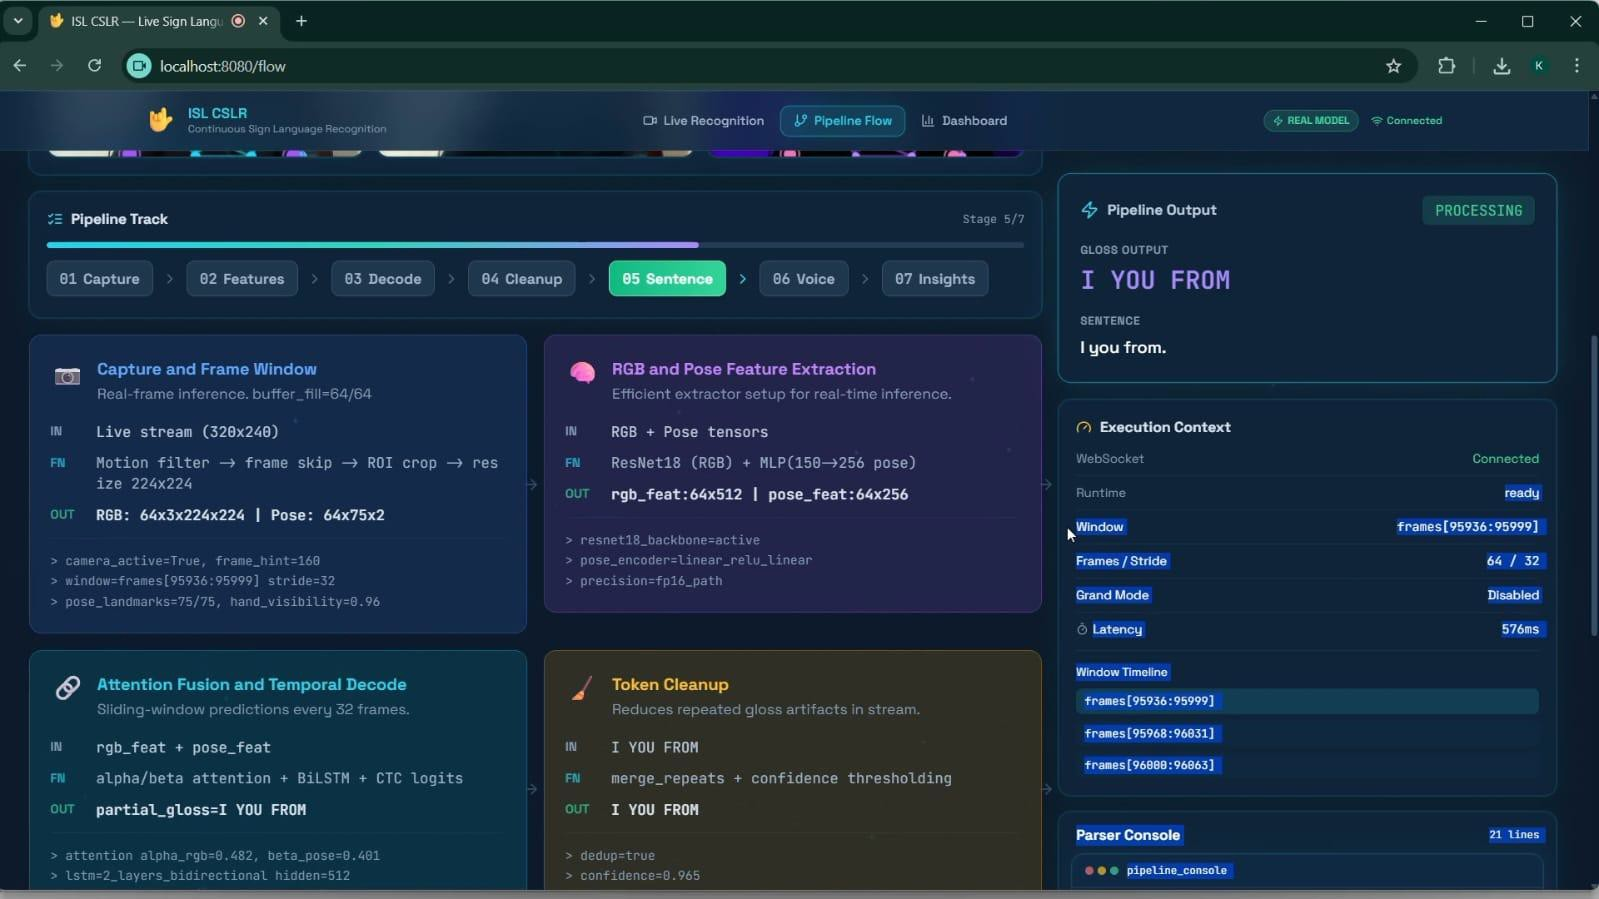
\includegraphics[width=0.9\textwidth]{text/figures/docx_image9.jpeg}
\caption{Intermediate output snapshot 2.}
\label{fig:intermediate-2}
\end{figure}

\subsection{Result Analysis}
\begin{itemize}[leftmargin=1.5em]
\item The current implementation shows reliable behavior for clear, well-segmented signs and short phrase-level cases in controlled real-time settings.
\item The configured low-latency operating target in the current test setup remains practical (reduced from reference behavior, but not aggressively minimized), preserving stability while keeping response time suitable for interaction.
\item Recognition confidence can fluctuate for rapid transitions, ambiguous articulation, or occluded hand motion, indicating expected sensitivity in challenging real-world inputs.
\item Moderate background variation is manageable, but performance remains dependent on capture quality, signer variability, and temporal consistency of incoming frames.
\item Overall, results support the project objective of a deployable CSLR baseline and provide a clear technical basis for subsequent optimization in data scale, decoding quality, and live robustness.
\end{itemize}

The above observations summarize the qualitative behavior of the current system under the tested real-time conditions.
